\chapter{Průvodce aplikací}
\label{Průvodce aplikací}


Po zadání webové adresy do administrátorského rozhraní se zobrazí přihlašovací okno. Pro úspěšné přihlášení musí být uživatel nastaven jako staff. 

\begin{figure}[H] \centering
  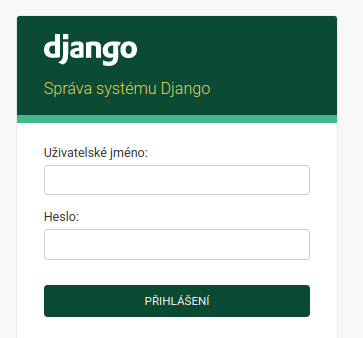
\includegraphics[width=200pt]{./pictures/50-prihlaseni.png}
    \caption[Přihlašování do administrátorské aplikace]{Přihlašování do administrátorské aplikace}
	\label{Přihlašování do administrátorské aplikace}                                
\end{figure}


Pokud se uživatel přihlásí jako administrátor (superuser), má přístup ke všem funkcím a tabulkám, které Django poskytuje. To je editování vzhledu stránky, přidávání, editování a mazání uživatelů a skupin a přístup do tabulky Cvut s přidruženými tabulkami.

\begin{figure}[H] \centering
  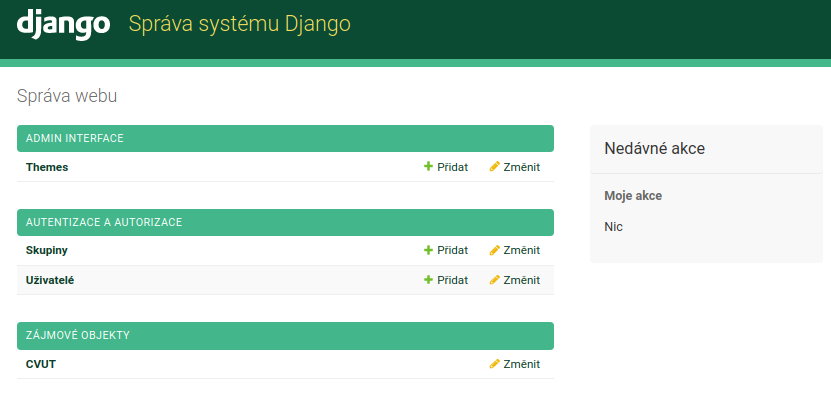
\includegraphics[width=420pt]{./pictures/51-mp-admin.png}
    \caption[Hlavní stránka pro přihlášení jako administrátor]{Hlavní stránka pro přihlášení jako administrátor}
	\label{Hlavní stránka pro přihlášení jako administrátor}                                
\end{figure}

\newpage

Zobrazení stránky pro uživatele, který má přístup pouze k tabulce Cvut.

\begin{figure}[H] \centering
  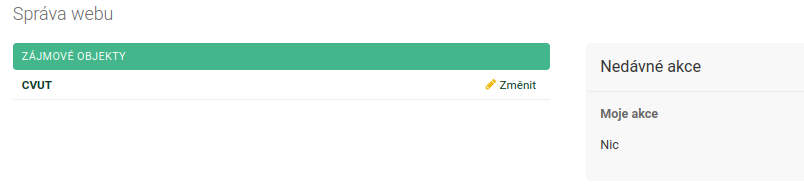
\includegraphics[width=320pt]{./pictures/58-uzivatel.png}
    \caption[Zobrazení stránky pro uživatele]{Zobrazení stránky pro uživatele}
	\label{Zobrazení stránky pro uživatele}                                
\end{figure}

Zobrazení tabulky Cvut s filtry a vyhledáváním.

\begin{figure}[H] \centering
  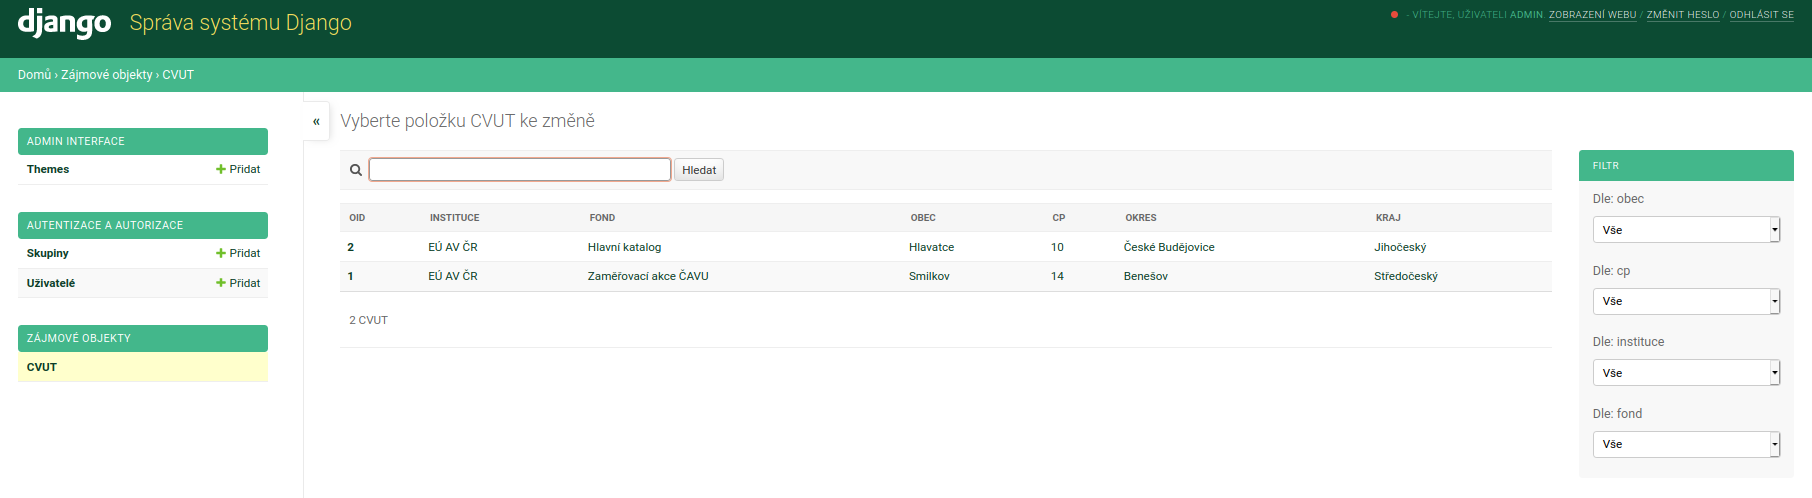
\includegraphics[width=420pt]{./pictures/52-cvut-admin.png}
    \caption[Hlavní stránka pro přihlášení jako administrátor]{Hlavní stránka pro přihlášení jako administrátor}
	\label{Hlavní stránka pro přihlášení jako administrátor}                                
\end{figure}


Po rozkliknutí záznamu se o něm zobrazí všechan data z tabulek Cvut, Base\_Images a CvutFiles. Superuživatelé mají možnost měnit práva k objektům pomocí tabulky Managers.

\begin{figure}[H] \centering
  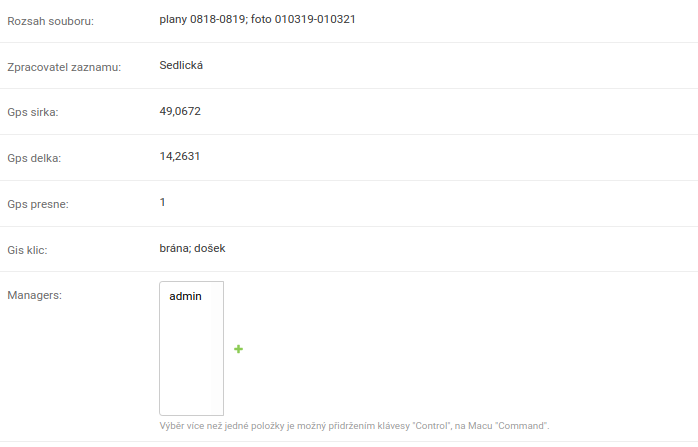
\includegraphics[width=340pt]{./pictures/53-data-managers.png}
    \caption[Zobrazení záznamu s možností měnit práva uživatelů]{Zobrazení záznamu s možností měnit práva uživatelů}
	\label{Zobrazení záznamu s možností měnit práva uživatelů}                                
\end{figure}


Zobrazení fotografií s náhledem z tabulky Base\_Images a souborů z tabulky CvutFiles. Možnost přidání a editace soubrů je možná, jen pokud k tomu má uživatel oprávnění.

\begin{figure}[H] \centering
  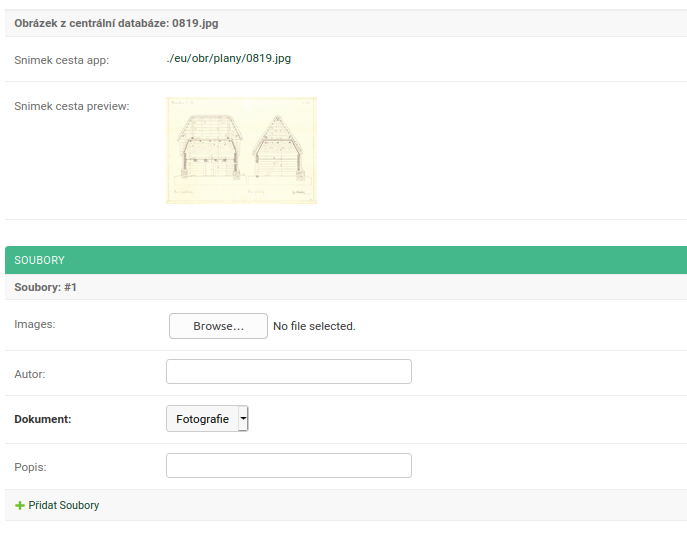
\includegraphics[width=320pt]{./pictures/54-obrazky.png}
    \caption[Zobrazení záznamu s možností měnit práva uživatelů]{Zobrazení záznamu s možností měnit práva uživatelů}
	\label{Zobrazení záznamu s možností měnit práva uživatelů}                                
\end{figure}


Po rozkliknutí \emph{Uživatelé} se zobrazí seznam všech uživatelů. Zde je možnost jejich editace, kde lze nastavit administrátorský přístup, superuživatele, zařadit uživatele do skupin nebo mu přiřadit jednotlivá práva.

\begin{figure}[H] \centering
  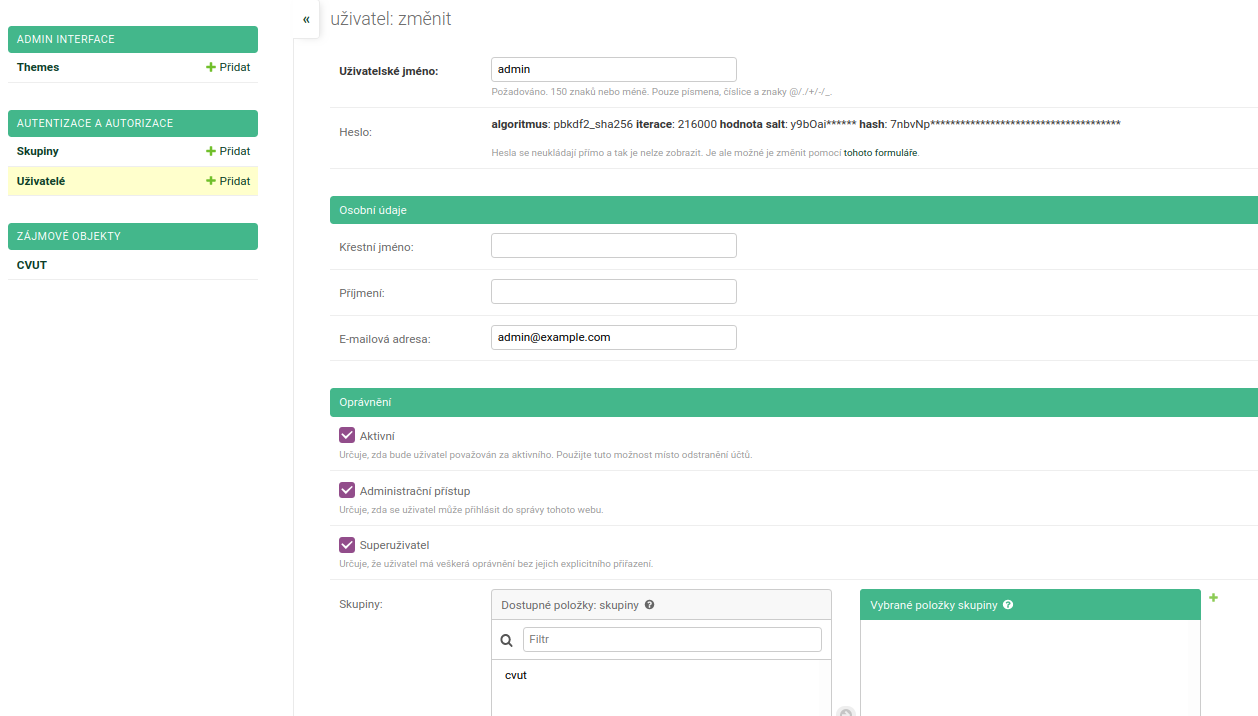
\includegraphics[width=390pt]{./pictures/55-sprava-uzivatelu.png}
    \caption[Správa uživatelů]{Správa uživatelů}
	\label{Správa uživatelů}                                
\end{figure}


Možnost nastavení skupin, u kterých lze navolit jednotlivá práva a poté do nich jednoduše přidávat uživatele.

\begin{figure}[H] \centering
  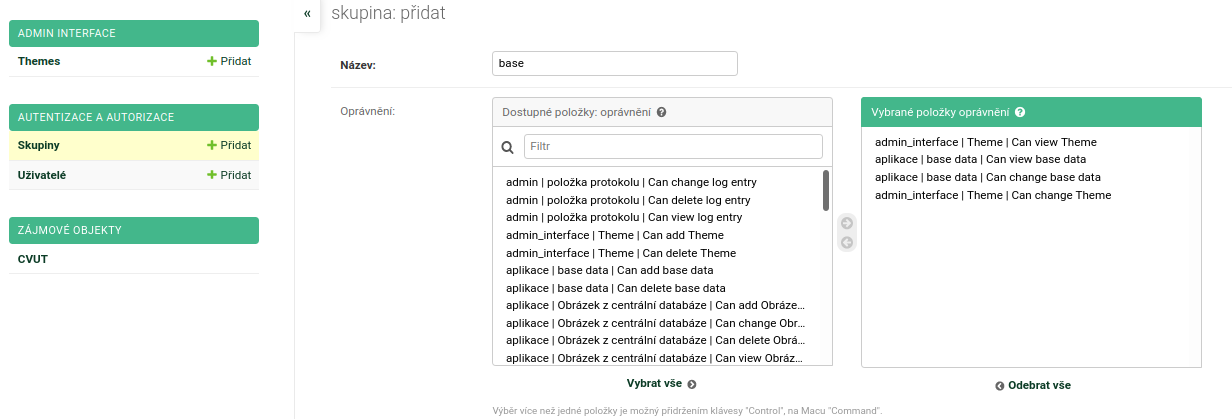
\includegraphics[width=420pt]{./pictures/56-skupiny.png}
    \caption[Tvorba skupin]{Tvorba skupin}
	\label{Tvorba skupin}                                
\end{figure}


V nastavení \emph{Theme} se může jednoduše měnit styl zobrazení stránky. Nastavit se dá například logo stránky, barva pozadí nebo textu.

\begin{figure}[H] \centering
  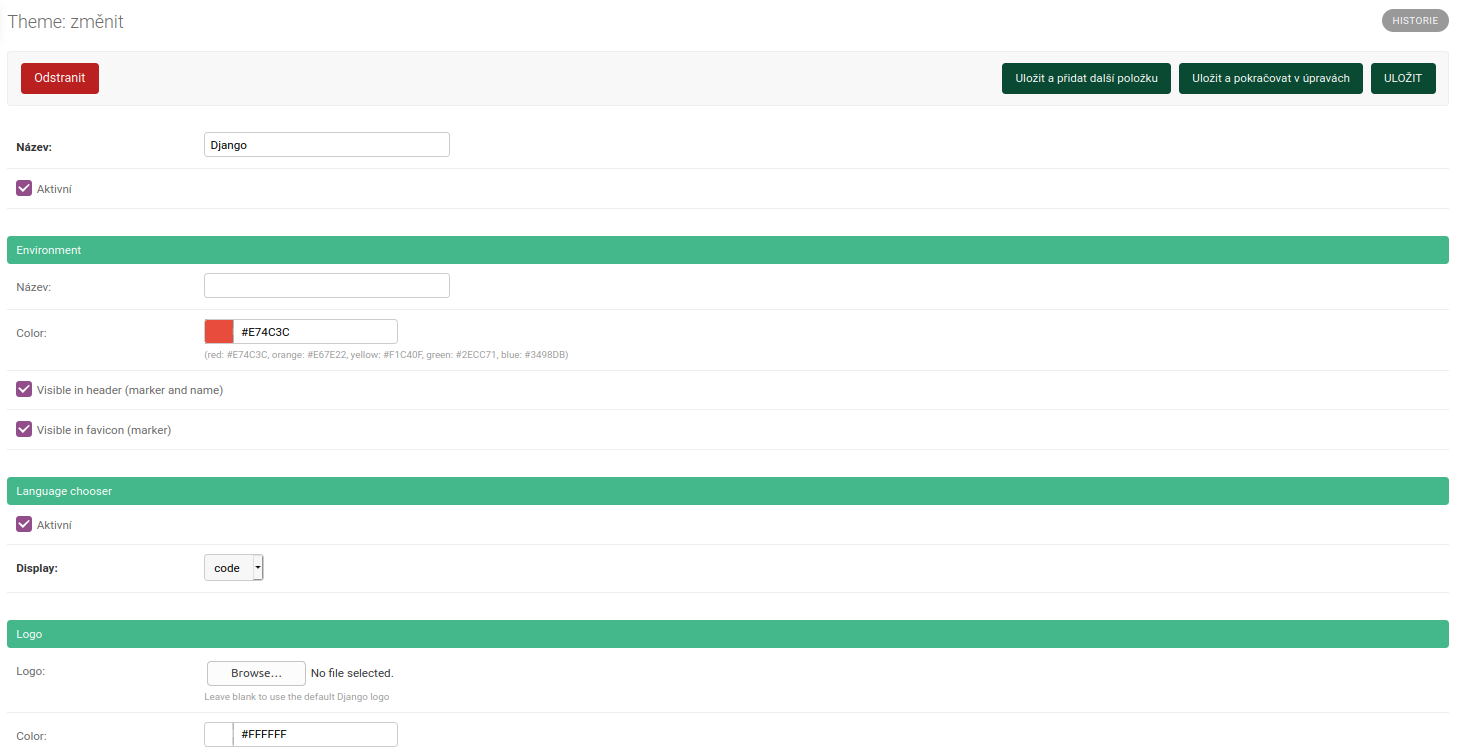
\includegraphics[width=420pt]{./pictures/57-theme.png}
    \caption[Nastavení vzhledu stránky]{Nastavení vzhledu stránky}
	\label{Nastavení vzhledu stránky}                                
\end{figure}



\chapter{Zdrojový kód}
\label{Zdrojový kód}

\begin{itemize}
	\item naki-viskalia.zip
\end{itemize}


